\documentclass[12pt]{article}
\parindent=0.25in

\setlength{\oddsidemargin}{0pt}
\setlength{\textwidth}{440pt}
\setlength{\topmargin}{0in}
\usepackage{amssymb}
\usepackage{amsfonts}
\usepackage{amsmath}
\usepackage{cancel}
\usepackage{latexsym}
\usepackage[center]{subfigure}
\usepackage{epsfig}
\usepackage{3952}
\usepackage{3952-thm}
\usepackage{pstricks,pst-node,pst-tree}
\usepackage{soul, xcolor}
\usepackage{bbold}
\usepackage[backref, colorlinks,citecolor=blue,bookmarks=true]{hyperref}  


% \def\size{\mathop{\rm{size}}\nolimits}
% \def\depth{\mathop{\rm{depth}}\nolimits}
% \newtheorem{theorem}{Theorem}
% \newtheorem{lemma}{Lemma}
% \newtheorem{corollary}{Corollary}
% \newtheorem{fact}{Fact}
% \newtheorem{definition}{Definition}
% \newtheorem{claim}{Claim}
% \newenvironment{proof}{\noindent \textbf{Proof:}}{$\Box$}
% \newenvironment{proofsketch}{\noindent \textbf{Proof Sketch:}}
% \newcommand{\infint}{\int_{-\infty}^\infty}
% \newcommand{\intunit}{\int_{-1}^1}
% \newcommand{\binclass}{x \in \{0,1\}^n}
% \newcommand{\example}{\textbf{Example:} }
% \newcommand{\observation}{\textbf{Observation:} }
% \newcommand{\note}{\textbf{Note:} }
% \newcommand{\noisy}[1]{N_\epsilon(#1)}
% \newcommand{\noisens}[1]{ns_\epsilon(#1)}
% \newcommand{\eg}{{\it e.g.,\ }}
% \newcommand{\Inf}{{\mathrm{Inf}}}
% \newcommand{\PAR}{{\mathrm{PAR}}}
% \def\poly{\mathop{\rm{poly}}\nolimits}
% \def\eps{{\epsilon}}
% \newcommand{\E}{{\bf E}}
% \def\through{{,\ldots,}}


\pagestyle{headings}    % Go for customized headings

\newcommand{\handout}[5]{
   \noindent
   \begin{center}
   \framebox{
      \vbox{
    \parbox[t]{4in} {\bf #1 } \vspace{3mm}  {\hfill \bf #2 }
       \vspace{2mm}
       \hbox to 6.00in { {\Large \hfill #5  \hfill} }
       \vspace{1mm}
       \hbox to 6.00in { {\it #3 \hfill #4} }
      }
   }
   \end{center}
   \vspace*{1mm}
}

\hypersetup{linkcolor=magenta}

\begin{document}

\handout{MATH 3952 (Undergraduate Seminar): Quantum Information Theory}{Spring 2024}
{Organizer: Patrick Lei; Presenter: Rimas Chacar-Palubinskas}
{Scribe: Mark Chen}{Lecture 2, Talk 2: February 5, 2024}

\thispagestyle{plain}
% \setcounter{section}{-1}
\section*{Chapter 2 (ctd): Qubits}
\section{Pauli Operators}
\begin{definition}[Pauli Gates $\&$ Clifford Gates]
We define the following as parts of a single circuit: $$
\underset{\text{Clifford Gates}}{\underbrace{\overset{H}{\overbrace{\frac{1}{\sqrt{2}}\begin{bmatrix}
1 & 1 \\
1 & -1
\end{bmatrix}}} \underset{\text{Pauli Gates}}{\underbrace{\overset{X, \sigma_x, \sigma_1}{\overbrace{\begin{bmatrix}
0 & 1\\
1 & 0
\end{bmatrix}}}\overset{Y, \sigma_y, \sigma_2}{\overbrace{\begin{bmatrix}
0 & -i\\
i & 0
\end{bmatrix}}}\overset{Z, \sigma_z, \sigma_3}{\overbrace{\begin{bmatrix}
1 & 0\\
0 & -1
\end{bmatrix}}}}}\overset{S}{\overbrace{\begin{bmatrix}
1 & 0\\
0 & i
\end{bmatrix}}}}}\overset{T}{\overbrace{\begin{bmatrix}
1 & 0\\
0 & e^{i\frac{\pi}{4}}
\end{bmatrix}}}
$$. For a bit of notations:
\begin{itemize}
    \item $X$ gate is just \underline{the $\NOT$ gate}, and it is also known as the \textbf{bit-flip operation}.
    \item $Z$ gate is what we have seen from the previous talk today of a phase shift gate with the phase shift being $\pi$. Recall that it was named a \textbf{phase flip operation}.
    \item $Y$ gate is just a product of $X$ and $Z$.
    \item We also mentioned $S$ and $T$ gates, which are also phase-shift gates with specific assignments of $\varphi$, $S$ with $\varphi = \frac{\pi}{2}$ and $T$ with $\varphi = \frac{\pi}{4}$.
\end{itemize}
\end{definition}

\begin{recall}
Recall what we have defined:
\begin{itemize}
    \item (Identity) $$
    \mathbb{1} = \begin{bmatrix}
        1 & 0\\
        0 & 1
    \end{bmatrix}
    $$
    \item (Bit-flip) $$
    X = \sigma_x = \begin{bmatrix}
        0 & 1\\
        1 & 0
    \end{bmatrix}
    $$
    \item (Bit-phase-flip) $$
    Y = \sigma_y = \begin{bmatrix}
        0 & -i\\
        i & 0
    \end{bmatrix}
    $$
    \item (Phase-flip) $$
    Z = \sigma_z = \begin{bmatrix}
        1 & 0\\
        0 & -1
    \end{bmatrix}
    $$
\end{itemize}
Next, we will show some identities of these Pauli operators / matrices to understand why they are so convenient.
\end{recall}

\begin{proposition}[Bit-Phase Flip]
We have already seen why $X$ and $Z$ flip bits and phases respectively. It is easy to see the identity that $$
ZX = iY
$$, which is the reason why $Y$ is called the \textbf{bit-phase flip}.
\end{proposition}

\begin{proposition}[Pauli matrices are unitary and Hermitian]
Recall the definition of these two:
\begin{itemize}
    \item (Hermitian) $U^\dag = U$.
    \begin{proof}
        Notice that, out of the four, only $X,Y$ have non-zero non-diagonal elements, and $X$'s non-diagonal elements are identical, which means $Y$ is the only Pauli matrix that may have a different conjugate transpose (i.e. image under $\dag$). So, we verify if $Y$ satisfies the Hermitian equality: $$
        Y^\dag = \begin{bmatrix}
            0 & -i\\
            i & 0
        \end{bmatrix}^\dag
        = \begin{bmatrix}
            0 & i^*\\
            -i^* & 0
        \end{bmatrix} = \begin{bmatrix}
            0 & -i\\
            i & 0
        \end{bmatrix} = Y
        $$, as desired.
    \end{proof}
    \item (Unitary) $U^\dag = U^{-1}$.
    \begin{proof}
        Since they are all Hermitian as shown, it is same as to prove they are their own inverse. But this is trivially true just by their definition (they are either flipping the bit or phase or both, so flipping twice obviously gets back to the original). We can also mathematically verify by actually checking $$
        X^2 = Y^2 = Z^2 = \mathbb{1}
        $$
    \end{proof}
    \item (Anti-Commutativity) It is easy to verify by multiplying out that, other than the identity matrix, we have pair-wise relationship as following:$$
    \begin{aligned}
    XY &= -YX\\
    XZ &= -ZX\\
    YZ &= -ZY
    \end{aligned}
    $$
\end{itemize}
\end{proposition}

\begin{remark}
The Pauli operators are also called \textbf{sigma operators} (usually when we use $\sigma_x, \sigma_y, \sigma_z$ to denote) or \textbf{Pauli spin matrices} (when written as matrices in the standard basis, as we have done).
\end{remark}

\begin{proposition}[Hadamard Gates Turn Phase-Flips into Bit-Flips, vice versa]\label{prop:flip-identities}
i.e.: $$
\begin{aligned}
HXH &= Z\\
HZH &= X
\end{aligned}
$$. Furthermore, it also has $$
HYH = -Y
$$
These show the important \textbf{interplay between Pauli operators and the Hadamard gates}, as well as the important identities for \textbf{quantum error corrections}.
\end{proposition}

\section{Single Qubit $\&$ Rotations in $3$D}
\subsection{Any unitary operation on a single qubit}
\textbf{Question:} How many real parameters does it take to specify one $n\times n$ matrix that takes values in $\CC$ that is unitary?
\begin{proposition}[$n^2$ is the answer!]\label{prop:pmtr-to-decide-map}
An $n\times n$ matrix has $n^2$ entries. Each entry is specified by two real numbers to uniquely identify a complex number, so $2n^2$ in total. But, since the matrix must be unitary, this restriction allows us to solve for this unique matrix using only $n^2$ real parameters.
\end{proposition}

\subsubsection{Now, let's look at the $2\times 2$ case specifically.}
By proposition \ref{prop:pmtr-to-decide-map}, we need $n^2$ real parameters to specify a complex $n\times n$ matrix, meaning that for $n=2$, we need $2^2 = 4$ real parameters. Now, if we further let the global phase factor to be ignored (due to equivalence up to global phase factor), then we actually only need $3$ real parameters to specify!

\begin{lemma}\label{lemma:circuit-for-all-2-by-2}
Any unitary operation on a qubit (up to global phase factor) can be implemented by a circuit containing two Hadamard gates and three phase gates:
\begin{center}
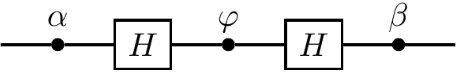
\includegraphics[width = 20em]{images/6.jpg}
\end{center}
\end{lemma}

\begin{theorem}\label{thm:single-qubit-circuit-general-form}
By lemma \ref{lemma:circuit-for-all-2-by-2}, all the real parameters we need to specify a unitary $2\times 2$ matrix is $\alpha, \varphi, \beta\in [0,2\pi]$, and the overall matrix for this general circuit is $$
U(\alpha, \beta, \varphi) = \begin{bmatrix}
e^{-i\prt{\frac{\alpha + \beta}{2}}}\cos\frac{\varphi}{2} & -ie^{i\prt{\frac{\alpha - \beta}{2}}}\sin\frac{\varphi}{2}\\
-ie^{-i\prt{\frac{\alpha - \beta}{2}}}\sin\frac{\varphi}{2} & e^{i\prt{\frac{\alpha + \beta}{2}}}\cos\frac{\varphi}{2}
\end{bmatrix}
$$
\end{theorem}

\subsection{The Bloch Sphere}
The theorem \ref{thm:single-qubit-circuit-general-form} is super important! Next, based on that theorem, we show how the set of all $2\times 2$ unitary matrices forms a non-abelian group under matrix multiplication, $U(2)$.

\begin{theorem}[$U(2)/U(1) \cong \SO(3)$]\label{thm:unitaries-to-rotation-iso}
That is, compositions of single-qubit unitaries $\cong$ (``behave the same as") compositions of rotations in three dimensions. This isomorphism helps us visualize the actions ofo single-qubit gates.
\end{theorem}
\begin{proof}
Recall the superposition of output of a quantum computation:$$
\begin{aligned}
\Ket{\psi}
    &= \alpha \Ket{0} + \beta \Ket{1}\\
    &= \cos\frac{\theta}{2} e^{i\varphi_0} \Ket{0} + \sin\frac{\theta}{2} e^{i\varphi_1} \Ket{1}
\end{aligned}
$$ [$\cos$ and $\sin$ are natural options because $|\alpha|^2 + |\beta|^2 = 1$; and there is a good reason why we use $\frac{\theta}{2}$ instead of $\theta$ which we will discuss later]. Finally, factor out the global factor gives us: $$
\Ket{\psi} = e^{i\varphi_0}\prt{\cos\frac{\theta}{2}  \Ket{0} + \sin\frac{\theta}{2} e^{i(\varphi_1 - \varphi_0)} \Ket{1}} = e^{i\varphi_0}\prt{\cos\frac{\theta}{2}  \Ket{0} + \sin\frac{\theta}{2} e^{i\varphi} \Ket{1}} \equiv \cos\frac{\theta}{2}  \Ket{0} + \sin\frac{\theta}{2} e^{i\varphi} \Ket{1}
$$, the last equivalence is because \underline{global phase factor} doesn't matter.

But this form is exactly the same as a vector on a sphere, which we call the \textbf{Bloch sphere}:
\begin{center}
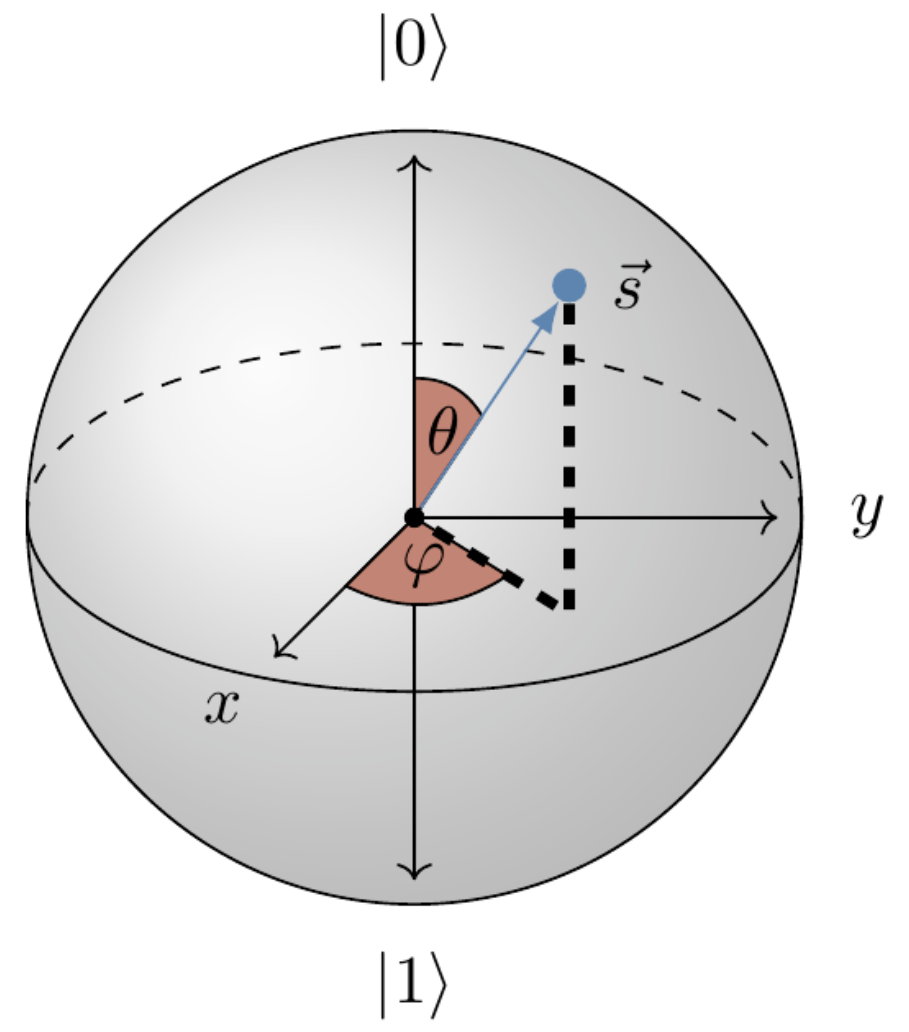
\includegraphics[width = 15em]{images/7.jpg}
\end{center}
Note that the $xy$-plane can be seen as the complex number coordinate, where $x$-axis is the real part axis, and $y$-axis is the imaginary part axis. It should be clear how there is a one-to-one relationship between $$
\cos\frac{\theta}{2}  \Ket{0} + \sin\frac{\theta}{2} e^{i\varphi} \Ket{1}
$$ and a point on the sphere.
\end{proof}

\begin{definition}[Bloch vector]
Use the figure from theorem \ref{thm:unitaries-to-rotation-iso}, we call the $\vec{s}$ which is specified by the two real parameters $\theta$ and $\varphi$ as the \textbf{Bloch vector}. Notice that, as the Bloch sphere is a unit sphere, any such $\vec{s}$ is a \underline{unit vector}.

Another way to look at the Bloch vector is such: Pauli matrices serve as a basis, so any operator can be expanded into the following form: $$
M = m_0\overset{=\mathbb{1}}{\overbrace{\sigma_0}} + \prt{m_x\sigma_x + m_y\sigma_y + m_z\sigma_z} = m_0\sigma_0 + \vec{m}\cdot \vec{\sigma}
$$
\end{definition}

\begin{corollary}\label{cor:unitary-to-rotation}
A corollary of theorem \ref{thm:unitaries-to-rotation-iso} is that any unitary action on the state vector will induce a rotation of the corresponding Bloch vector.
\end{corollary}
\begin{proof}
Since there is a bijection between the unitary group after its actions and a Bloch vector, such actions will simply rotate the original Bloch vector.
\end{proof}

\subsection{A natural question to ask based off of corollary \ref{cor:unitary-to-rotation} is what kind of rotation are we talking about?}
The complete answer will be given in chapter 3, but now, we can give some simple ones that are easy to get by hand calculations for intuitions first.

\begin{proposition}\label{prop:orth-state-vec-on-bloch}
Any two orthogonal state vectors appear on the Bloch sphere as two Bloch vectors pointing in opposite directions.
\end{proposition}
\begin{proof}
A single yet slightly irresponsible proof lies in the fact that the, in the expression of $U$, the zenith angle is halved (as for why, don't worry about it). Particularly, we know that for a unitary matrix, the eigenvectors are perpendicular, where there is an angle of $\frac{\pi}{2}$ between them. But this corresponds to an angle $$
\frac{\theta}{2} = \frac{\pi}{2}\implies \theta = \pi
$$, meaning that the two eigenvectors are parallel and point to the opposite directions.
\end{proof}

\begin{proposition}
Following proposition \ref{prop:orth-state-vec-on-bloch} and recalling that two eigenvectors of a single-qubit unitary $U$ are always orthogonal, we know that such eigenvectors define an axis through the center of the Bloch sphere, and so we denote such an axis as the $\vec{n}$ on the block sphere. Equationally, we can express any such unitary map as $$
U = \cos\frac{\alpha}{2} \mathbb{1} + i\vec{n}\cdot \vec{\sigma} \sin\frac{\alpha}{2}
$$, where:
\begin{itemize}
    \item $\alpha$ parametrizes the angular velocty of the angular rotation of $\vec{s}$ about $\vec{n}$. This can be acquired from the eigenvalues of $U$, which equal to $$
    e^{\mp i\alpha/2}\text{ up to a global phase factor}
    $$
    \item $\vec{n}$ parametrizes the axis about which the Bloch vector rotates.
    \item $\vec{\sigma}$ is the Pauli basis.
\end{itemize}
So, this way, it makes clear the way how $U$, as an action, makes $\vec{s}$ rotate.
\end{proposition}

\begin{example}[$P_\alpha\prt{\cos\frac{\theta}{2}\Ket{0} + e^{i\varphi}\sin\frac{\theta}{2}\Ket{1}} = \cos\frac{\theta}{2}\Ket{0} + e^{i(\varphi + \alpha)}\sin\frac{\theta}{2}\Ket{1}$]
That is, we change the azimuthal angle from $\varphi$ to $\varphi + \alpha$. This is the same as rotatin the Bloch sphere anticlockwise by $\alpha$ about the $z$-axis.
\end{example}

\begin{example}[$\vec{\sigma}$]
We can describe what each component of the $\vec{\sigma}$ does:
\begin{itemize}
    \item $\sigma_z$: Rotation of $\pi$ about the $z$-axis, becuase it has a eigenvectors of $Z = \Ket{0}$ and $-Z = \Ket{1}$
    \item $\sigma_x$: With eigenvectors of $\frac{\Ket{0} \pm \Ket{1}}{\sqrt{2}}$, rotation by $\pi$ about $x$-axis.
    \item $\sigma_y$: With eigenvectors of $\frac{\Ket{0} \pm i\Ket{1}}{\sqrt{2}}$, rotation by $\pi$ about $y$-axis.
    \item Hadamard: Combining the identities we have shown in proposition \ref{prop:flip-identities} and $H^2 = 1$ (giving its eigenvalues of $\pm1$), we can decide that it represents \hl{rotation by $\pi$ about the diagonal $(x+z)$-axis}.
\end{itemize}
\end{example}

\begin{proposition}
We will show that, in general, a unitary $U$ is given by $$
U(s_x X + s_y Y + s_z Z) U^\dag = s'_xX + s'_yY + s_z'Z
$$, showcasing how quantum operations are equivalent to geometric rotations on the Bloch sphere.
\end{proposition}

\subsection{Composition of Rotations}
Recall the
\begin{center}
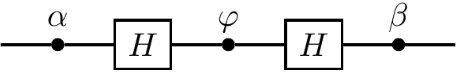
\includegraphics[width = 15em]{images/6.jpg}
\end{center}
that we have seen before. This corresponds to what we have concluded in subsection 2.3. That is, we have
\begin{enumerate}
    \item The first phase gate to rotate by $\alpha$ about the $z$-axis.
    \item The second phase gate to rotate by $\varphi$ about the $x$-axis.
    \item The third phase gate to rotate by $\beta$ about the $z$-axis.
\end{enumerate}

Since any unitary $U$ can be described by such rotations, we can implement any unitary $U$ by choosing the three phase shifts, $\alpha, \varphi$, and $\beta$.

\begin{proposition}[The above process is generally true for any unitary $2\times 2$ actions]
Any rotations can be achieved by the above three rotations in that order. So, any unitary operations can be constructed as such.
\end{proposition}

\begin{remark}
One thing to notice is that it is hard to make the unitary operations precise. Since Bloch sphere is a continuous space as we have shown, it is a good idea to consider approximations to this unitary operations.
Suppose that we want to approximate the $U$ circuit we want with some $\widetilde{U}$ circuit, and $$
U = U_1U_2\ldots U_k\ldots U_N; \widetilde{U} = \widetilde{U_1}\widetilde{U_2}\ldots \widetilde{U_k}\ldots \widetilde{U_N}
$$ are both series of gates. Then, we denote that $$
||\widetilde{U}_k - U_k|| \leq \delta_k
$$, then $$
||\widetilde{U} - U|| \leq \underset{k}{\sum}\delta_k
$$. Then, to achieve, suppose each difference are all $\delta$, $$
||\widetilde{U} - U|| \leq \epsilon \implies N\delta \leq \epsilon\implies \delta \leq \frac{\epsilon}{N}
$$

Finally, suppose $P$ is the output superposition of $U$, and $\widetilde{P}$ of $\widetilde{U}$. Then, $||\widetilde{P} - P||\leq 2\epsilon$.
\end{remark}

\end{document}